\chapter{Predictive Modelling and Evaluation}\label{ch:models}

This chapter answers the predictive question, \emph{what is likely to happen next?} It covers the four
analytical problems in turn: demand forecasting, large-order classification, segmentation and anomaly detection.

\section{Monthly demand forecasting}
\subsection{Set-up}
The forecasting panel contains \PanelSeries products observed monthly. There are \PanelTrain training rows
(2020--2024) and \PanelTest test rows (January 2025 -- September 2026). Each model predicts
$\log(1+\text{units})$, and the prediction is converted back to units. The log scale suits the multiplicative
nature of demand and stops the largest products from dominating the fit. Seven algorithms were tuned by
randomised search over the expanding-window folds described in \cref{ch:method}. \Cref{tab:hyper} in
\cref{app:hyper} lists the selected hyper-parameters.

\subsection{One-step-ahead results}
\Cref{tab:forecast} reports test performance when each month is forecast with the actual history up to the
previous month. This is the operational scenario of a monthly planning cycle. Every machine-learning model
clearly beats both naive baselines. The best model, \BestReg, reaches RMSE \BestRegRMSE units, WAPE
\BestRegWAPE\% and $R^2=\BestRegRtwo$. That is an RMSE \GainVsSNaive\% lower than the seasonal-naive rule
(\SNaiveRMSE) and \GainVsNaive\% lower than the naive rule (\NaiveRMSE).

\begin{table}[htbp]
\centering
\footnotesize
\caption{Monthly product-demand forecasting: test-set performance (one-step-ahead, Jan 2025--Sep 2026)}
\label{tab:forecast}
\begin{adjustbox}{max width=\linewidth}
\begin{tabular}{lrrrrrrrr}
\toprule
\textbf{Model} & \textbf{MAE} & \textbf{MSE} & \textbf{RMSE} & \textbf{R$^2$} & \textbf{MAPE \%} & \textbf{WAPE \%} & \textbf{CV RMSE} & \textbf{Fit (s)} \\
\midrule
Seasonal naive (same month last year) & 120.0 & 23,233 & 152.4 & 0.551 & 15.38 & 14.74 & -- & 0.0 \\
Naive (last month) & 139.8 & 31,051 & 176.2 & 0.400 & 18.00 & 17.17 & -- & 0.0 \\
Support Vector Regression & 90.6 & 13,271 & 115.2 & 0.744 & 12.26 & 11.13 & 0.2151 & 24.9 \\
Linear Regression & 91.3 & 13,861 & 117.7 & 0.732 & 11.48 & 11.21 & 0.1691 & 0.2 \\
XGBoost & 93.3 & 14,294 & 119.6 & 0.724 & 12.28 & 11.46 & 0.1917 & 94.8 \\
Random Forest & 93.0 & 14,413 & 120.1 & 0.722 & 12.04 & 11.42 & 0.1918 & 142.6 \\
Gradient Boosting & 95.7 & 15,113 & 122.9 & 0.708 & 12.51 & 11.76 & 0.1889 & 124.9 \\
K-Nearest Neighbors & 97.0 & 15,865 & 126.0 & 0.694 & 12.01 & 11.91 & 0.1951 & 6.8 \\
Decision Tree & 103.6 & 17,978 & 134.1 & 0.653 & 13.70 & 12.73 & 0.2077 & 8.1 \\
\bottomrule
\end{tabular}
\end{adjustbox}
\par\smallskip\parbox{0.92\linewidth}{\footnotesize\emph{Note:} Errors in units per product-month. CV RMSE is the mean validation RMSE on the log scale over the expanding-window folds 2022, 2023 and 2024 used for tuning. Baselines need no fitting.}
\end{table}

Three further observations stand out. First, the differences between the better models are small. RMSE values
range only from \BestRegRMSE to \WorstRegRMSE units, and linear regression on log features (\LinRMSE) is
competitive with the tree ensembles (random forest \RFRMSE, XGBoost \XGBRMSE). Once good lag and seasonal
features exist, the problem is largely log-linear, and model complexity adds little. This agrees with
\citet{makridakis2018}. Second, the single decision tree is the weakest learner (\DTRMSE), as expected from its
high variance; averaging many trees in a forest removes most of this weakness \citep{breiman2001}. Third, the
cross-validated scores on the training years rank the models similarly to the test scores. The validation
design therefore gives a reliable guide to future performance. \Cref{fig:forecastcomp} compares the models and
shows that predictions of \BestReg track the actual values closely across products of very different size.

\begin{figure}[htbp]\centering
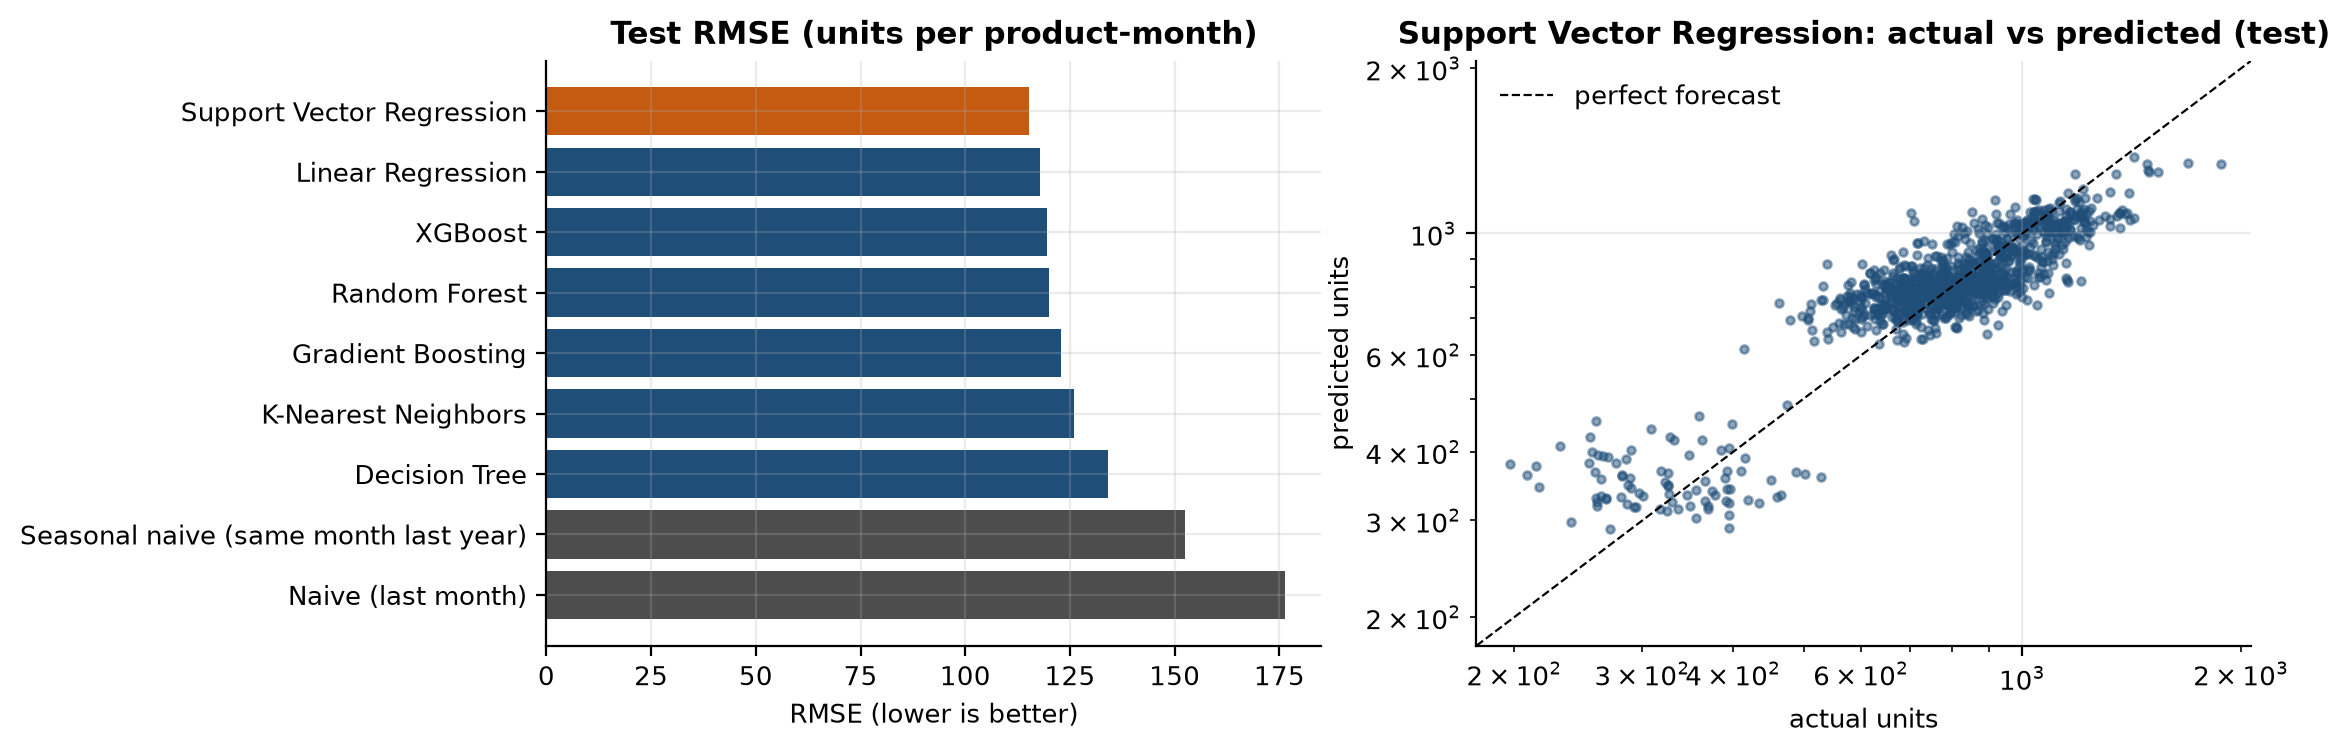
\includegraphics[width=\linewidth]{ml_forecast_comparison}
\caption{Test RMSE of all forecasting models (left; best model highlighted, baselines in grey) and actual versus predicted units for the best model (right)}\label{fig:forecastcomp}
\end{figure}

\subsection{Recursive multi-step results}
A harder test is to forecast all 21 test months from December 2024 \emph{without} seeing any actual data after
training. Each month's predictions are fed back in as history for the next month. This is the scenario of an
annual budget. \Cref{tab:recursive} shows that the best models degrade only modestly. \BestRec achieves a
WAPE of \BestRecWAPE\% ($R^2=\BestRecRtwo$), still far better than repeating the 2024 pattern. XGBoost degrades
the most under recursion. Errors compound when a model's own predictions become inputs, and boosted trees, which
fit the training data closely, are more exposed to this.

\begin{table}[htbp]
\centering
\small
\caption{Recursive 21-month forecast from December 2024 (no actual data used after training)}
\label{tab:recursive}
\begin{adjustbox}{max width=\linewidth}
\begin{tabular}{lrrrrr}
\toprule
\textbf{Model} & \textbf{MAE} & \textbf{RMSE} & \textbf{R$^2$} & \textbf{MAPE \%} & \textbf{WAPE \%} \\
\midrule
Random Forest & 91.0 & 117.0 & 0.736 & 11.85 & 11.18 \\
Support Vector Regression & 92.3 & 117.2 & 0.735 & 12.65 & 11.34 \\
Linear Regression & 94.1 & 121.4 & 0.715 & 11.73 & 11.56 \\
XGBoost & 104.1 & 137.5 & 0.635 & 16.17 & 12.79 \\
Seasonal naive (2024 pattern repeated) & 125.9 & 158.1 & 0.517 & 15.87 & 15.47 \\
\bottomrule
\end{tabular}
\end{adjustbox}
\end{table}

\subsection{Company-level forecasting and model reconciliation}
Product forecasts can be summed to a company total and compared with statistical models fitted directly to the
total series (\cref{tab:company}, \cref{fig:companyfc}). At this aggregate level, the Holt--Winters model with
additive trend and multiplicative seasonality is the most accurate, with a MAPE of only \HWMAPE\%. The summed
machine-learning forecasts are also accurate but slightly less so. The result is consistent with the literature:
smooth aggregate series favour statistical models, while the cross-learning ability of machine learning pays
off at the level of individual products. The framework therefore combines the two through \emph{top-down
reconciliation} \citep{athanasopoulos2009}. Holt--Winters sets the company total and its prediction interval,
and the machine-learning model distributes that total across products. Product plans then add up exactly to the
company plan.

\begin{table}[htbp]
\centering
\small
\caption{Company-level monthly units forecast, test period Jan 2025--Sep 2026}
\label{tab:company}
\begin{adjustbox}{max width=\linewidth}
\begin{tabular}{lrrr}
\toprule
\textbf{Model (company-total monthly units)} & \textbf{MAE} & \textbf{RMSE} & \textbf{MAPE \%} \\
\midrule
Holt-Winters (additive trend, multiplicative season) & 559 & 698 & 1.32 \\
SARIMA(1,1,1)(0,1,1)$_{12}$ on log units & 687 & 806 & 1.65 \\
Support Vector Regression one-step, summed over products & 712 & 875 & 1.68 \\
Random Forest recursive, summed over products & 1,186 & 1,386 & 2.77 \\
Seasonal naive (2024 repeated) & 2,549 & 2,817 & 6.00 \\
\bottomrule
\end{tabular}
\end{adjustbox}
\end{table}

\begin{figure}[htbp]\centering
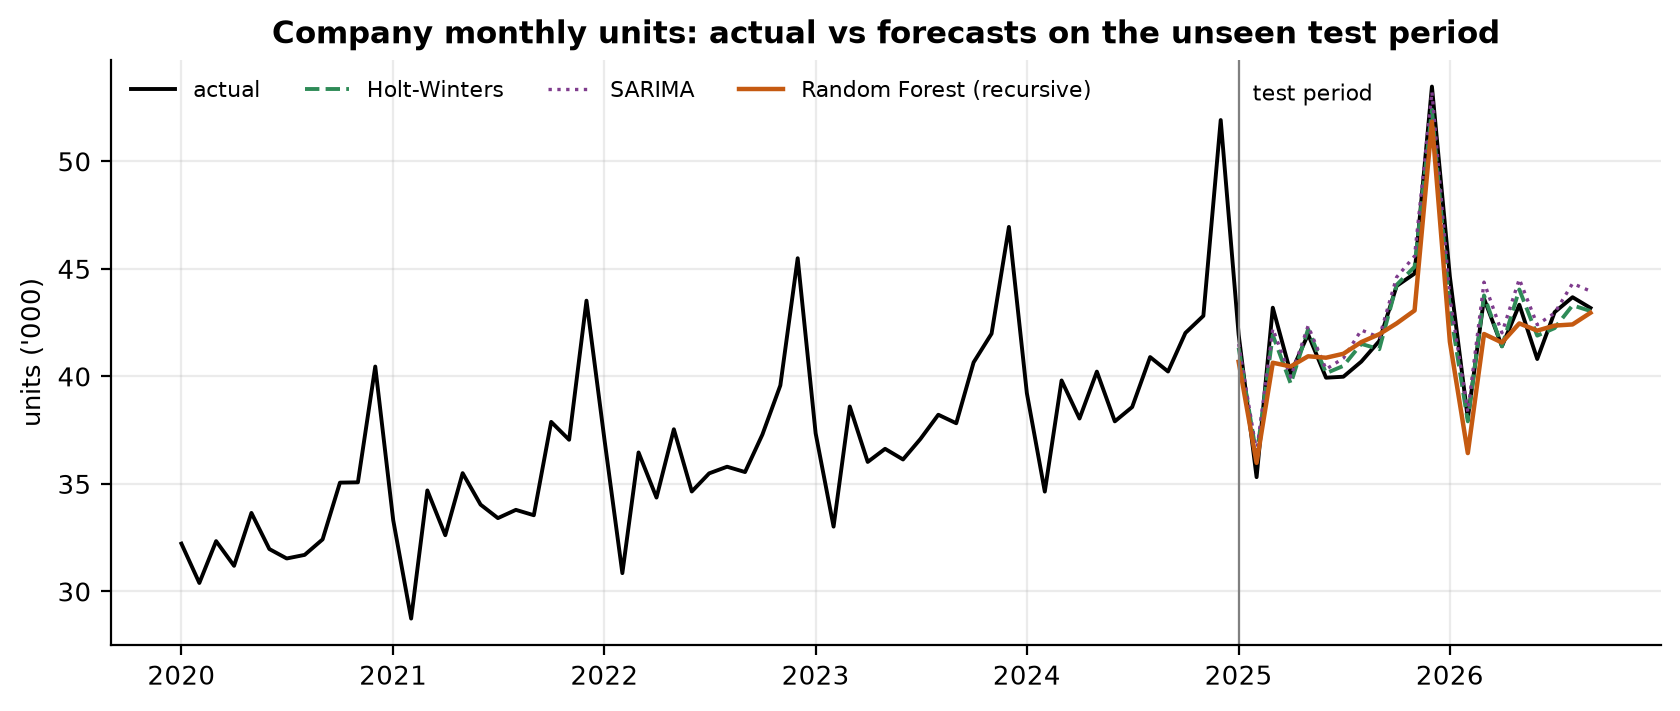
\includegraphics[width=\linewidth]{ml_company_forecast_test}
\caption{Company monthly units: actual values and competing forecasts over the test period}\label{fig:companyfc}
\end{figure}

\subsection{What drives the forecasts?}
\Cref{fig:importance} explains the models. For \BestReg, permutation importance shows that recent history
(lags and rolling means) carries most of the information, followed by seasonal features. The XGBoost SHAP values
give the same picture and also highlight the December indicator and the 12-month lag, which capture the
seasonal peak. The price features have little influence. This matches the near-zero price elasticity found in
\cref{ch:eda}, so the models and the explanatory analysis tell a consistent story.

\begin{figure}[htbp]\centering
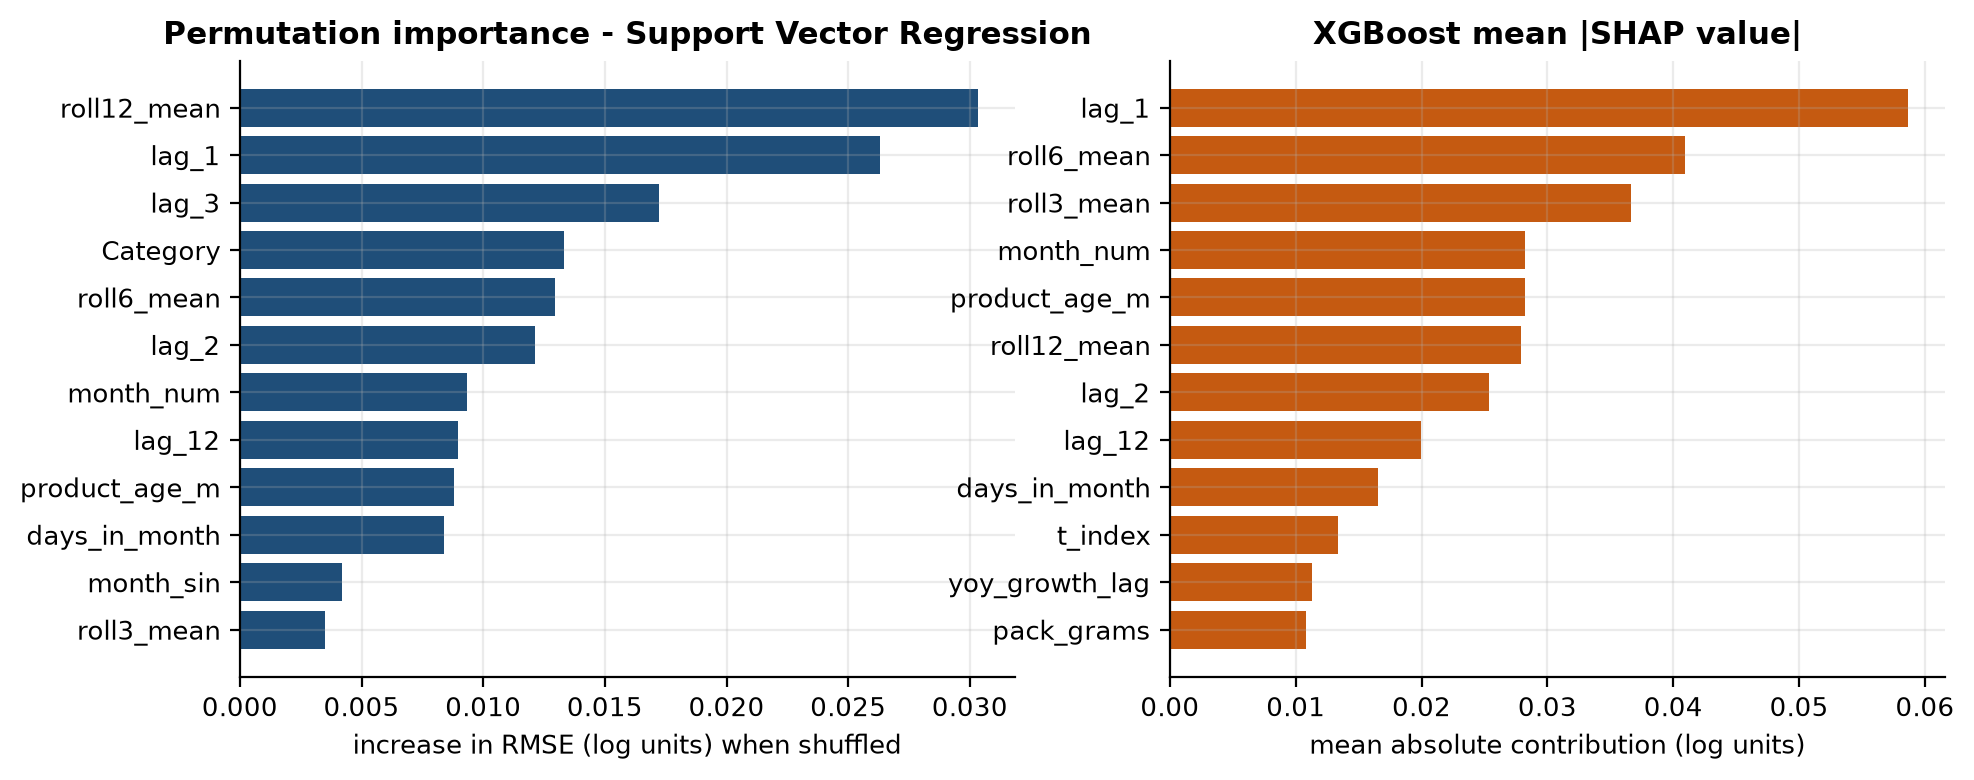
\includegraphics[width=\linewidth]{ml_feature_importance}
\caption{Permutation importance for the best forecasting model (left) and mean absolute SHAP values for XGBoost (right)}\label{fig:importance}
\end{figure}

\subsection{Twelve-month outlook}
The selected models were refitted on all data up to September 2026 and used to forecast October 2026 --
September 2027 (\cref{tab:future}, \cref{fig:future}). Net sales for these twelve months are forecast at
\BDT\FutSales million, with an 80\% interval from \FutSalesLo to \FutSalesHi million. That is \FutGrowth\% more
than the previous twelve months (\BDT\PrevSales million). Units are expected to change by \FutUnitsGrowth\%, and
the December peak is expected to recur. \FutTopCategory remains the largest category in the forecast. This
outlook can feed directly into the production, procurement and budgeting processes.

\begin{table}[htbp]
\centering
\footnotesize
\caption{Twelve-month forward forecast, October 2026 -- September 2027}
\label{tab:future}
\begin{adjustbox}{max width=\linewidth}
\begin{tabular}{lrrrrrrr}
\toprule
\textbf{Month} & \textbf{Units ML raw} & \textbf{Units (final)} & \textbf{80\% low} & \textbf{80\% high} & \textbf{Net sales (M)} & \textbf{80\% low } & \textbf{80\% high } \\
\midrule
Oct 2026 & 43,531 & 46,203 & 45,021 & 47,478 & 6.08 & 5.83 & 6.34 \\
Nov 2026 & 44,109 & 47,015 & 45,744 & 48,272 & 6.19 & 5.90 & 6.47 \\
Dec 2026 & 53,219 & 54,939 & 53,383 & 56,313 & 7.27 & 6.89 & 7.63 \\
Jan 2027 & 43,375 & 45,461 & 44,209 & 46,738 & 6.58 & 6.22 & 6.95 \\
Feb 2027 & 37,348 & 39,411 & 38,347 & 40,460 & 5.68 & 5.36 & 6.02 \\
Mar 2027 & 43,561 & 45,883 & 44,660 & 47,104 & 6.56 & 6.16 & 6.96 \\
Apr 2027 & 41,747 & 43,288 & 42,136 & 44,485 & 6.21 & 5.83 & 6.62 \\
May 2027 & 43,224 & 45,767 & 44,576 & 47,013 & 6.44 & 6.02 & 6.88 \\
Jun 2027 & 41,784 & 43,454 & 42,324 & 44,667 & 6.16 & 5.75 & 6.61 \\
Jul 2027 & 42,815 & 44,111 & 42,962 & 45,304 & 6.27 & 5.84 & 6.74 \\
Aug 2027 & 42,884 & 45,082 & 43,902 & 46,342 & 6.46 & 5.99 & 6.95 \\
Sep 2027 & 43,340 & 44,976 & 43,746 & 46,142 & 6.38 & 5.89 & 6.88 \\
\bottomrule
\end{tabular}
\end{adjustbox}
\par\smallskip\parbox{0.92\linewidth}{\footnotesize\emph{Note:} Units ML raw = sum of the Random Forest product forecasts before reconciliation. Final totals come from Holt-Winters models of company units and net sales (BDT million); intervals are the 10th and 90th percentiles of 2,000 simulated future paths. Product forecasts are scaled to these totals.}
\end{table}

\begin{figure}[htbp]\centering
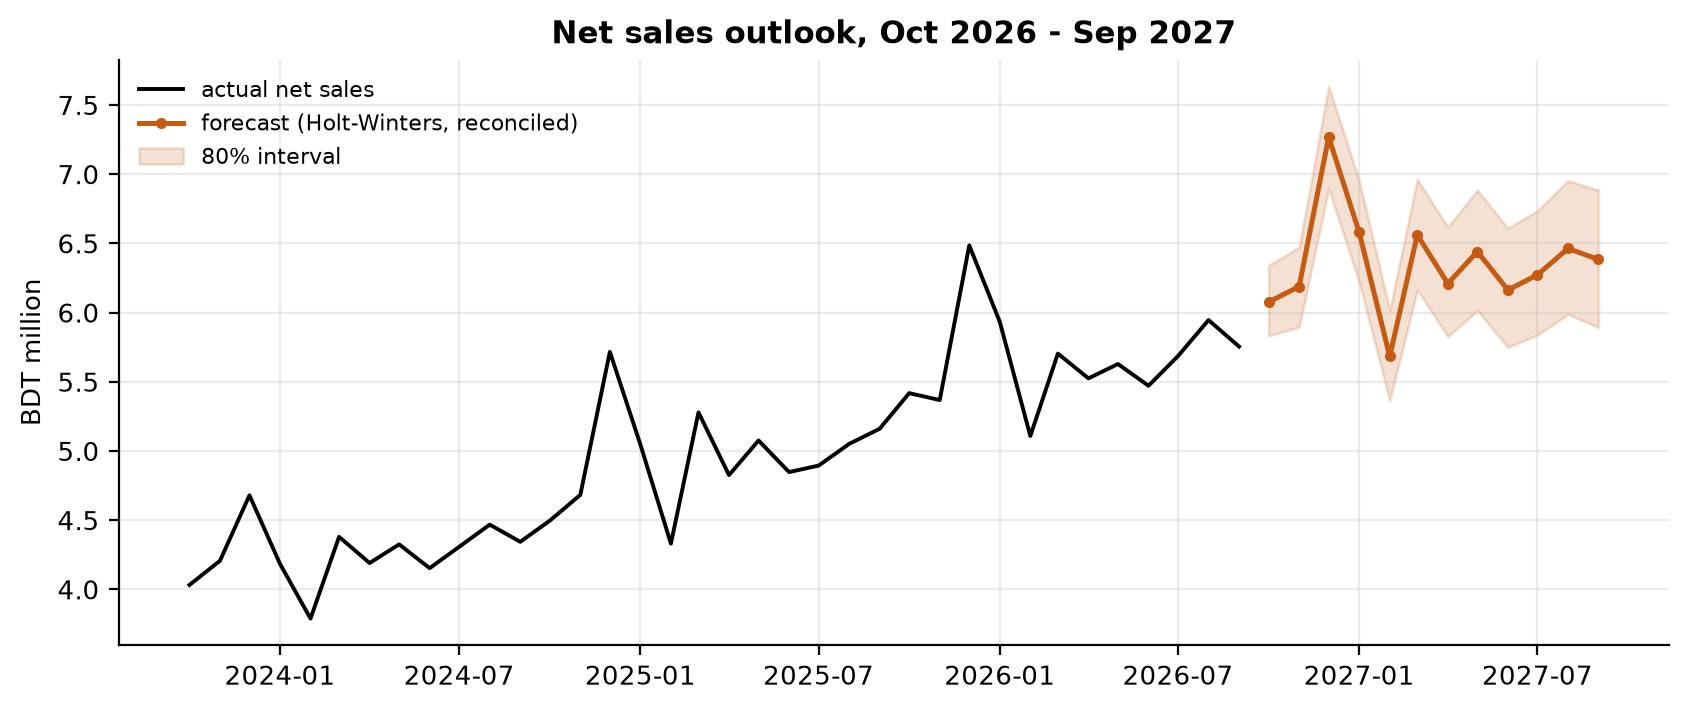
\includegraphics[width=\linewidth]{ml_future_forecast}
\caption{Net sales outlook for October 2026 -- September 2027 with 80\% prediction interval}\label{fig:future}
\end{figure}

\section{Large-order classification}
The classifier predicts, from information available when an order is entered, whether the order will contain
at least 10 units. Large orders made up \ClsPosTrain\% of training orders and \ClsPosTest\% of test orders. The
models were trained on \ClsTrain orders (2020--2024) and tested on \ClsTest orders (2025--2026). The features
were channel, region, customer type, category, price, discount, pack size, product age and calendar variables,
plus smoothed target encodings of channel $\times$ region and of product.

\begin{table}[htbp]
\centering
\footnotesize
\caption{Large-order classification ($\geq$10 units): test-set performance, 2025--2026}
\label{tab:classification}
\begin{adjustbox}{max width=\linewidth}
\begin{tabular}{lrrrrrrrrr}
\toprule
\textbf{Model} & \textbf{Accuracy} & \textbf{Precision} & \textbf{Recall} & \textbf{F1} & \textbf{ROC-AUC} & \textbf{PR-AUC} & \textbf{Threshold} & \textbf{Lift@10\%} & \textbf{Time (s)} \\
\midrule
Logistic Regression & 0.661 & 0.357 & 0.628 & 0.455 & 0.712 & 0.418 & 0.62 & 2.35 & 15 \\
Support Vector Machine (linear) & 0.629 & 0.341 & 0.698 & 0.458 & 0.711 & 0.417 & 0.31 & 2.34 & 42 \\
Gradient Boosting (hist) & 0.709 & 0.387 & 0.502 & 0.437 & 0.711 & 0.418 & 0.23 & 2.34 & 35 \\
Random Forest & 0.628 & 0.341 & 0.701 & 0.459 & 0.710 & 0.418 & 0.51 & 2.33 & 252 \\
XGBoost & 0.635 & 0.343 & 0.676 & 0.455 & 0.709 & 0.416 & 0.20 & 2.34 & 60 \\
Decision Tree & 0.550 & 0.309 & 0.807 & 0.447 & 0.709 & 0.407 & 0.48 & 2.31 & 14 \\
K-Nearest Neighbors & 0.634 & 0.333 & 0.624 & 0.434 & 0.684 & 0.396 & 0.20 & 2.28 & 73 \\
\bottomrule
\end{tabular}
\end{adjustbox}
\par\smallskip\parbox{0.92\linewidth}{\footnotesize\emph{Note:} Positive rate in the test years: 22.5\%; a classifier that always predicts `not large' would reach 77.5\% accuracy, so accuracy alone is misleading. Thresholds maximise F1 on the 2024 validation year. KNN uses a 60,000-row training sample. Lift@10\% is the large-order rate among the 10\% highest-scored orders divided by the overall rate.}
\end{table}

\Cref{tab:classification} and \cref{fig:classification} show a clear and instructive result. All seven
algorithms reach almost the same ROC-AUC, between \ClsAUCmin and \ClsAUC, and \ClsBest is the best. The model
that always predicts ``not large'' would be \ClsMajority\% accurate yet useless. The tuned models instead
recover most large orders (recall about \ClsRecall for \ClsBest) at moderate precision. Ranked by score, the top
10\% of orders contain large orders \ClsLift times more often than average. The ceiling is set by the
\emph{information} in the data, not by the algorithm. XGBoost (\ClsXGBAUC) gains nothing over logistic
regression, and KNN (\ClsKNNAUC) is weakest because distances become uninformative over many one-hot features.

\begin{figure}[htbp]\centering
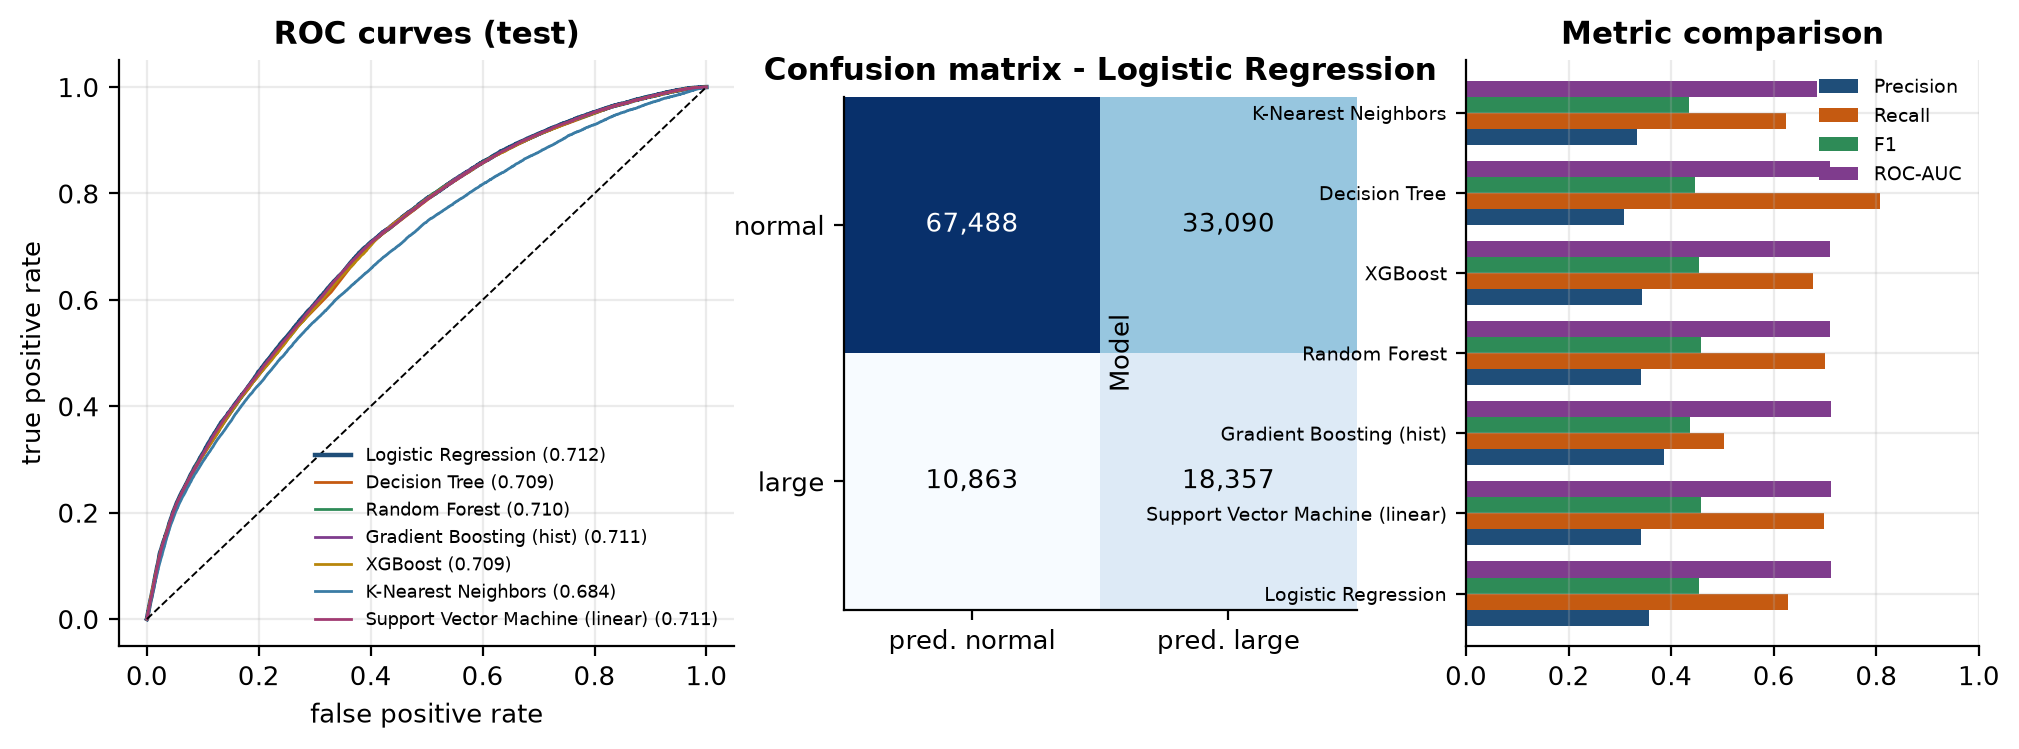
\includegraphics[width=\linewidth]{ml_classification}
\caption{ROC curves (left), confusion matrix of the best model (centre) and metric comparison (right) for large-order classification}\label{fig:classification}
\end{figure}

The XGBoost gain importance (\cref{fig:clsimp}) identifies the reason. The sales channel accounts for about
\ClsChannelImp\% of the model's gain and region for about \ClsRegionImp\%. Product, price, discount and
calendar contribute very little. In the test years \LargeDist\% of distributor orders were large, against only
\LargeEcom\% of E-commerce orders. Order size within a channel and region is otherwise close to random. For
decision-making, then, the useful output is a \emph{channel-and-region-level} expectation of large orders for
logistics planning, rather than a precise order-by-order prediction.

\begin{figure}[htbp]\centering
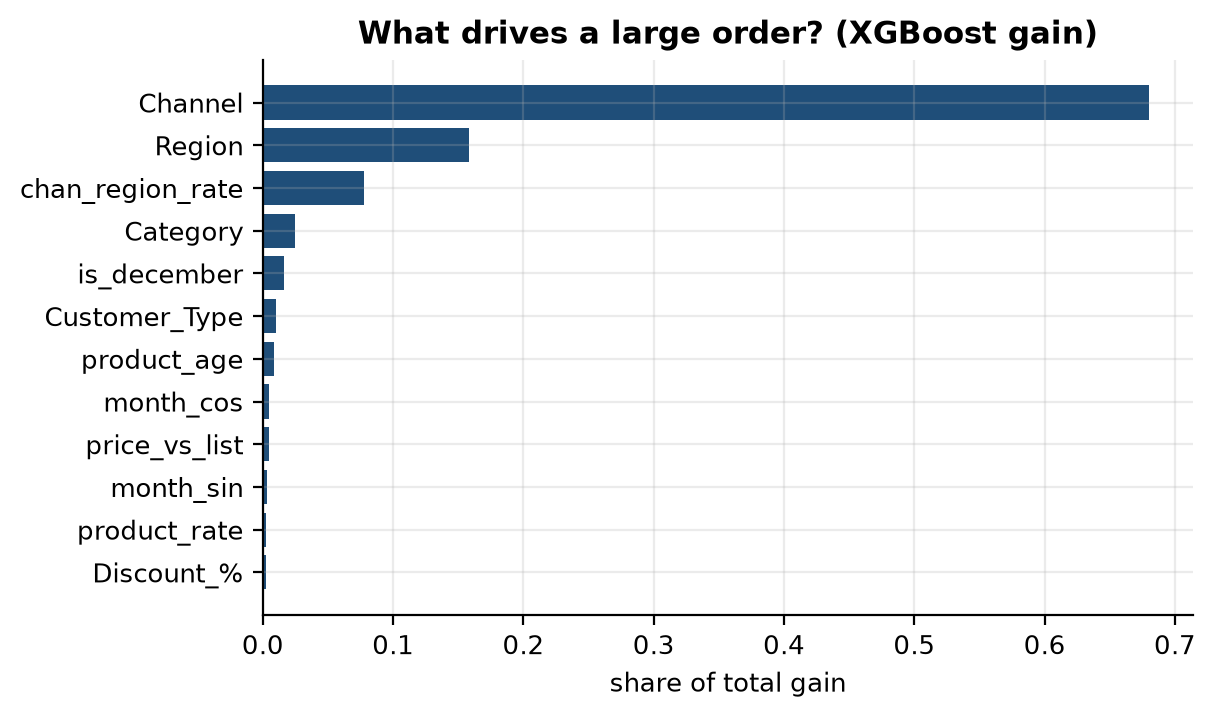
\includegraphics[width=.65\linewidth]{ml_classification_importance}
\caption{Drivers of large orders: XGBoost gain aggregated by original variable}\label{fig:clsimp}
\end{figure}

\section{Segmentation}
\subsection{Product portfolio}
Each product was described by its log revenue, log average price, unit growth from 2023 to 2025, December
seasonality index and month-to-month volatility. Order size and channel mix were excluded because they barely
vary between products (\cref{ch:eda}) and would only add noise. The features were standardised. $K$-Means,
agglomerative (Ward) and Gaussian-mixture clustering were compared for $k=2,\dots,8$
(\cref{fig:clustering}, \cref{tab:clustercompare}). Within the practical range of three to five segments,
$K$-Means with $k=\ProdK$ gave the best silhouette (\ProdSil) and a Davies--Bouldin index of \ProdDB. The
resulting segments are summarised in \cref{tab:productclusters} and named automatically from their averages.

\begin{table}[htbp]
\centering
\small
\caption{Product portfolio segments (K-Means, k=5)}
\label{tab:productclusters}
\begin{adjustbox}{max width=\linewidth}
\begin{tabular}{lrrrrrr}
\toprule
\textbf{Segment} & \textbf{Products} & \textbf{Sales share \%} & \textbf{Avg price} & \textbf{Units/order} & \textbf{Unit growth \%/yr} & \textbf{Dec. index} \\
\midrule
Premium \& gift packs & 13 & 33.3 & 156 & 6.24 & +7.8 & 123 \\
Mature slow-growth lines & 13 & 31.9 & 130 & 6.17 & +2.3 & 120 \\
Core family packs & 11 & 28.1 & 133 & 6.17 & +4.9 & 134 \\
Single-serve value packs & 9 & 4.2 & 23 & 6.22 & +6.0 & 119 \\
Niche \& new lines & 6 & 2.5 & 24 & 6.22 & +4.0 & 134 \\
\bottomrule
\end{tabular}
\end{adjustbox}
\par\smallskip\parbox{0.92\linewidth}{\footnotesize\emph{Note:} Growth is the compound annual growth of units between 2023 and 2025. December index = average December units relative to the product's average month (100 = no seasonality).}
\end{table}

\subsection{Market segments}
The 220 combinations of region, channel and customer type were clustered on their revenue, average order
value, units per order, price, discount, growth and gift-pack share. $K$-Means selected $k=\MktK$ segments
(silhouette \MktSil). They separate clearly into \emph{core retail trade} (General and Modern Trade in the large
cities), \emph{bulk distribution}, small-ticket \emph{online and regional} cells, and a group of
\emph{emerging high-growth} cells (\cref{tab:marketclusters}).

\begin{table}[htbp]
\centering
\scriptsize
\caption{Market segments of region $\times$ channel $\times$ customer-type cells (K-Means, k=4)}
\label{tab:marketclusters}
\begin{adjustbox}{max width=\linewidth}
\begin{tabular}{lrrrrrll}
\toprule
\textbf{Segment} & \textbf{Cells} & \textbf{Sales share \%} & \textbf{AOV (BDT)} & \textbf{Units/order} & \textbf{Growth \%/yr} & \textbf{Main channels} & \textbf{Main regions} \\
\midrule
Core retail trade & 99 & 71.9 & 518 & 5.02 & +14.8 & General Trade, Modern Trade & Dhaka, Chattogram, Gazipur \\
Bulk distribution & 52 & 22.6 & 966 & 9.96 & +16.2 & Distributor & Chattogram, Dhaka, Gazipur \\
Small-ticket online \& regional & 50 & 4.2 & 341 & 3.43 & +16.7 & E-commerce, Modern Trade & Barishal, Khulna, Rajshahi \\
Emerging high-growth cells & 19 & 1.3 & 431 & 4.16 & +33.2 & E-commerce, Modern Trade & Cumilla, Khulna, Mymensingh \\
\bottomrule
\end{tabular}
\end{adjustbox}
\end{table}
\begin{table}[htbp]
\centering
\small
\caption{Comparison of clustering algorithms at the selected number of clusters}
\label{tab:clustercompare}
\begin{adjustbox}{max width=\linewidth}
\begin{tabular}{llrrrr}
\toprule
\textbf{Problem} & \textbf{Algorithm} & \textbf{k} & \textbf{Silhouette} & \textbf{Davies-Bouldin} & \textbf{Calinski-Harabasz} \\
\midrule
Products & K-Means & 5 & 0.237 & 1.271 & 16.2 \\
Products & Agglomerative (Ward) & 5 & 0.212 & 1.195 & 14.9 \\
Products & Gaussian Mixture & 5 & 0.233 & 1.237 & 15.3 \\
Market cells & K-Means & 4 & 0.243 & 1.497 & 54.2 \\
Market cells & Agglomerative (Ward) & 4 & 0.250 & 1.467 & 48.9 \\
Market cells & Gaussian Mixture & 4 & 0.165 & 1.753 & 42.4 \\
\bottomrule
\end{tabular}
\end{adjustbox}
\par\smallskip\parbox{0.92\linewidth}{\footnotesize\emph{Note:} Higher silhouette and Calinski--Harabasz and lower Davies--Bouldin values indicate better-separated clusters.}
\end{table}

\begin{figure}[htbp]\centering
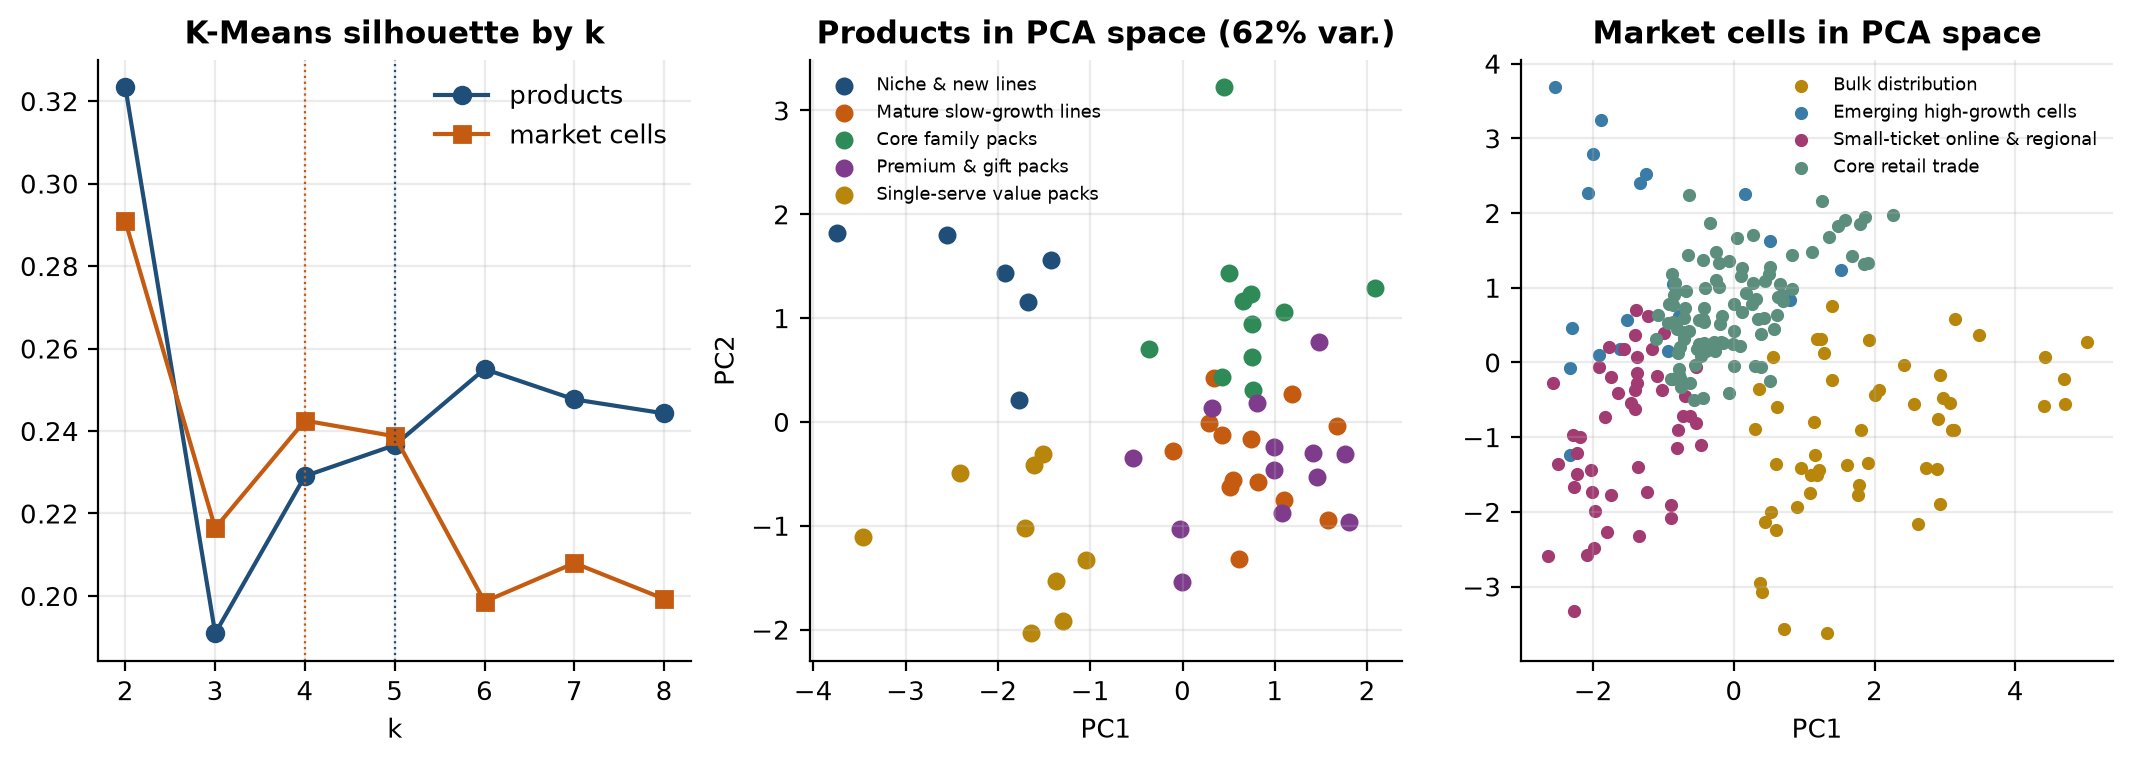
\includegraphics[width=\linewidth]{ml_clustering}
\caption{Silhouette score by number of clusters (left); products (centre) and market cells (right) projected onto the first two principal components}\label{fig:clustering}
\end{figure}

The silhouette values (\ProdSil and \MktSil) indicate weak to moderate structure \citep{rousseeuw1987}. The
segments are therefore useful summaries for strategy, not sharply separated natural groups. $K$-Means and Ward
clustering agreed closely, while Gaussian mixtures performed worst on these small samples. This ranking is
reported so that a reader can judge the robustness of the segmentation.

\section{Anomaly detection}
\subsection{Daily monitoring}
For each day, an expected value was computed as a 31-day centred rolling median multiplied by the month-of-year
seasonal factor. Deviations were scored on the log scale with the robust $z$-score
$z = 0.6745\,(r-\tilde r)/\text{MAD}$ and, separately, with an Isolation Forest over four daily features.
Together the two methods flagged \AnomDays of the 2,465 trading days: \AnomDaysZ by the robust $z$-score and
\AnomDaysIF by the Isolation Forest (\cref{fig:anomdaily}, \cref{tab:dailyanom}). Most flagged days are
unusually weak trading days. In a live deployment each would be checked against known causes such as public
holidays, strikes or system outages.

\begin{figure}[htbp]\centering
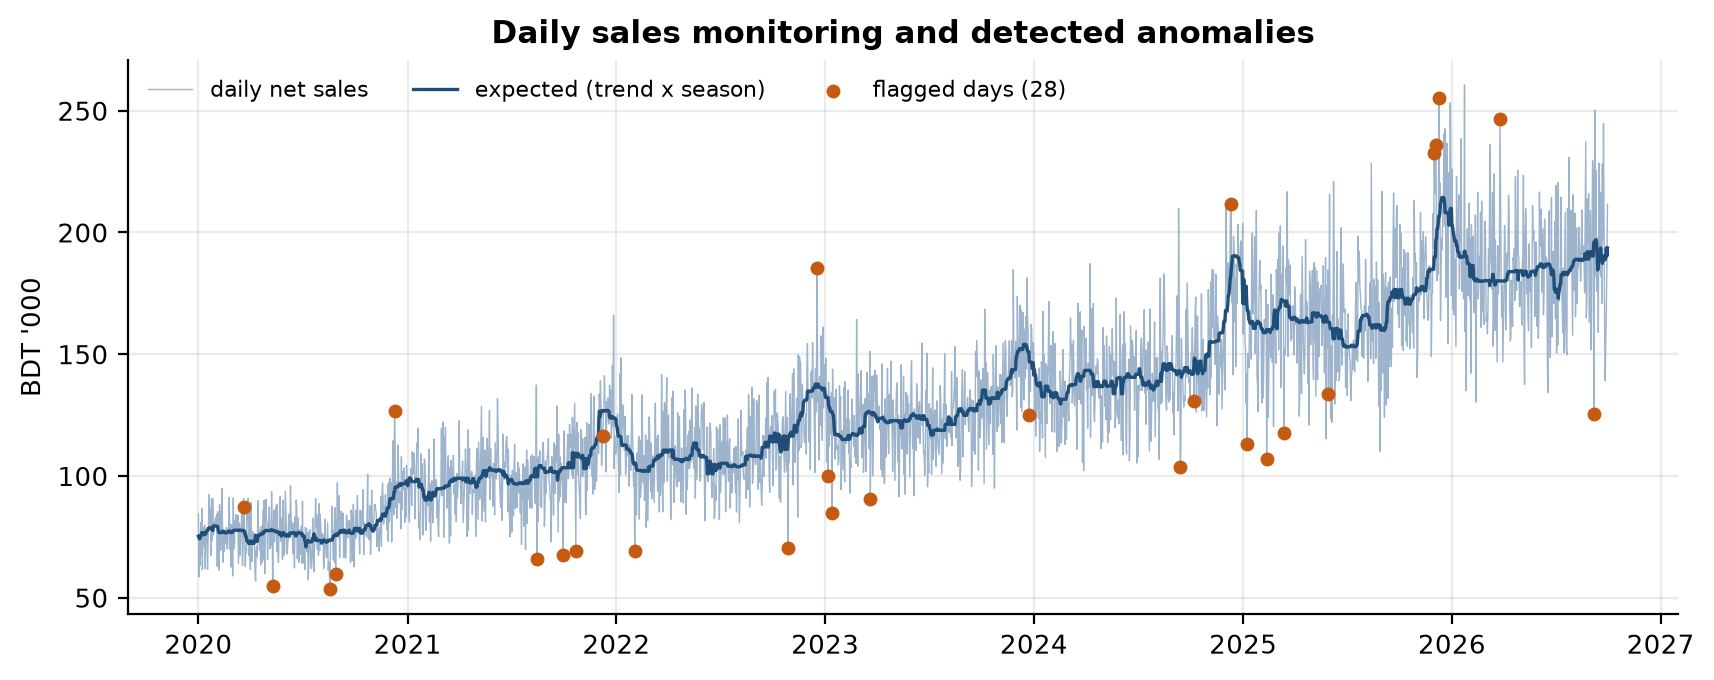
\includegraphics[width=\linewidth]{anomaly_daily}
\caption{Daily net sales, expected level and detected anomalies}\label{fig:anomdaily}
\end{figure}
\begin{table}[htbp]
\centering
\small
\caption{Ten most unusual trading days (seasonally adjusted)}
\label{tab:dailyanom}
\begin{adjustbox}{max width=\linewidth}
\begin{tabular}{lrrrrl}
\toprule
\textbf{Date} & \textbf{Net sales (BDT)} & \textbf{Expected (BDT)} & \textbf{Deviation \%} & \textbf{Robust z} & \textbf{Flagged by} \\
\midrule
28 Oct 2022 & 70,215 & 113,462 & -38.1 & -4.01 & robust z \\
22 Oct 2021 & 69,194 & 109,276 & -36.7 & -3.82 & robust z \\
06 Sep 2026 & 125,262 & 195,913 & -36.1 & -3.74 & robust z \\
30 Sep 2021 & 67,358 & 103,385 & -34.8 & -3.58 & both \\
02 Feb 2022 & 69,149 & 104,763 & -34.0 & -3.47 & Isolation Forest \\
15 Aug 2021 & 66,039 & 99,664 & -33.7 & -3.44 & Isolation Forest \\
11 Feb 2025 & 106,843 & 160,093 & -33.3 & -3.38 & Isolation Forest \\
13 Jan 2023 & 84,814 & 126,483 & -32.9 & -3.34 & Isolation Forest \\
08 Jan 2025 & 113,188 & 168,043 & -32.6 & -3.31 & Isolation Forest \\
13 Mar 2025 & 117,699 & 171,855 & -31.5 & -3.17 & Isolation Forest \\
\bottomrule
\end{tabular}
\end{adjustbox}
\end{table}

\subsection{Transaction screening}
Without labelled errors, a detector's ability cannot be measured on the real data. Following the approach of
the preprocessing scripts, 1,000 realistic errors of four types (250 each) were therefore planted in a copy of
the 500,000 orders (\cref{tab:anomaly}). The per-product IQR rule on quantity detected only \AnomIQRRecall\% of
the planted errors, because three of the four error types do not involve quantity. Simple business rules on
price and discount caught \AnomRuleRecall\% with perfect precision but missed every quantity error. The
Isolation Forest caught \AnomIFRecall\% across all four types. Price and discount errors were found completely,
and most inflated quantities were found too. The lesson is that rules and machine learning are complementary.
Rules are precise for known failure modes, and the Isolation Forest provides broad coverage for unknown ones.

\begin{table}[htbp]
\centering
\footnotesize
\caption{Detection of 1,000 injected transaction errors in 500,000 orders}
\label{tab:anomaly}
\begin{adjustbox}{max width=\linewidth}
\begin{tabular}{lrrrrrrr}
\toprule
\textbf{Method} & \textbf{Flagged} & \textbf{Precision} & \textbf{Recall} & \textbf{Price x10} & \textbf{Qty x20} & \textbf{Disc. 30-45\%} & \textbf{Price 10\%} \\
\midrule
IQR on log quantity (per product) & 1,500 & 0.112 & 0.168 & 0.00 & 0.66 & 0.00 & 0.01 \\
Business rules (price, discount) & 750 & 1.000 & 0.750 & 1.00 & 0.00 & 1.00 & 1.00 \\
Isolation Forest (4 features) & 2,500 & 0.364 & 0.909 & 1.00 & 0.64 & 1.00 & 1.00 \\
Rules OR Isolation Forest & 2,500 & 0.364 & 0.909 & 1.00 & 0.64 & 1.00 & 1.00 \\
\bottomrule
\end{tabular}
\end{adjustbox}
\par\smallskip\parbox{0.92\linewidth}{\footnotesize\emph{Note:} The last four columns give the share of each error type that was detected. 250 errors of each type were planted in a copy of the data.}
\end{table}

\section{Summary of model evaluation}
\begin{table}[htbp]\centering\small
\caption{Summary of the selected model for each analytical problem}\label{tab:modelsummary}
\begin{tabularx}{\linewidth}{@{}lXl@{}}
\toprule
\textbf{Problem} & \textbf{Selected approach} & \textbf{Key test result} \\ \midrule
Product demand (1-step) & \BestReg & WAPE \BestRegWAPE\%, $R^2$ \BestRegRtwo \\
Product demand (multi-step) & \BestRec, recursive & WAPE \BestRecWAPE\% \\
Company total & Holt--Winters + top-down reconciliation & MAPE \HWMAPE\% \\
Large orders & \ClsBest & ROC-AUC \ClsAUC, lift \ClsLift \\
Product segments & $K$-Means, $k=\ProdK$ & silhouette \ProdSil \\
Market segments & $K$-Means, $k=\MktK$ & silhouette \MktSil \\
Transaction anomalies & rules OR Isolation Forest & recall \AnomComboRecall\% \\ \bottomrule
\end{tabularx}
\end{table}
As the proposal required, models were selected on appropriate metrics \emph{and} business relevance, not on
accuracy alone. Where a simpler model performed as well as a complex one, as with logistic regression versus
XGBoost for classification, the simpler and more interpretable model is preferred.
